\chapter{Numerical experiments} \label{chap:numerical-experiments}

% ~~~~~~~~~~~~~~~~~~~~~~~~~~~~~~~~~~~~~~~~~~~~~~~~~~~~~~~~~~~~~~~~~~~~~~~~~~~~~~~~~~~~~~~~~~~~~~~~~~~~~~~~~~~
\section{Setup} \label{sec:numerical-experiments/setup}

In this section, we will present benchmark instances used for evaluating the proposed methods and algorithms,
we will describe the modification process for creating problem instances suited to our studied problem,
briefly describe how we model the problem in the constraint programming model,
as described in \cref{sec:problem-statement/constraint-programming-model},
and how we obtain (near) optimal solutions to the modeled problem using a constraint programming solver.

All processing described in the following sections was done in Python using a library
developed specifically for the purposes of this thesis.
More about the library and running the following experiments can be found in \cref{sec:attachments/documentation}.

% -----------------------------------------------------------------------------------------------------------
\subsection{Problem instances} \label{subsec:numerical-experiments/setup/instances}

\citet{Kolisch1997} created the PSPLIB%
\footnote{Available online at \url{https://www.om-db.wi.tum.de/psplib/}}
--- set of benchmark instances for the \ac{rcpsp}.
This set has since been used to evaluate and compare many results in the literature.
(For example, some recent papers from \citet{Bianco2011}, \citet{Cheng2015}, or \citet{Elsayed2017}.)

We will use and modify specific instances from the PSPLIB single-mode instance set.
Instances from this set model the standard \ac{rcpsp}.
They consist of 30, 60, 90, or 120 jobs
and 4 renewable resources with fixed capacities.
Each job has an execution duration and consumption requirements for each of the resources defined.
Precedences between jobs are stated, forming a single-component precedence graph.
The goal when scheduling such problem instances is usually minimizing the project makespan,
or minimizing the project tardiness with respect to a specified project due date.

To fully model the studied problem, we introduce several modifications to the original instances.
Namely, we split the precedence graph to create individual order components,
introduce job deadlines and time-variable resource capacities,
and to maintain feasibility when modeling specific production systems
we scale down job durations and resource consumptions.
Following are the modification steps in more detail.

Initially, to model a system with fewer resources than the original 4,
we remove the undesired resources from the problem instance
and optionally adjust the resource consumption of jobs.
If by removing all resources consumed by a job,
which in turn is left with no required consumption,
the total removed consumption is distributed among the remaining resources.
We then continue with modifications common for all instances.

First, we split the single-component precedence graph into disconnected components,
creating an inforest.
We do this by ordering the jobs topologically
and selecting one of the last topological generations as seed jobs%
\footnote{The depth of the selected generation influences the number of created components
and the overall structure of the created intree forest.}.
Incrementally, starting with the preceding generation
and continuing in the reverse order of topological generations,
each job from preceding generations selects a single successor precedence
to connect to a successor job.
Analogously, each job from succeeding generations selects a single predecessor precedence
to connect to a predecessor job.
After splitting the graph into an inforest,
the sink-roots of the intrees are selected as orders $\Orders$.

Second, we limit the resource availabilities to simulate working shifts.
The capacity function of a resource is a combination of periodical shift availability
and later introduced capacity changes, in the form of capacity additions and migrations.
We use periodical availability intervals, sub-intervals of $\intinterval{1}{24}$,
to denote that a resource is available each day during the specified time intervals.
During those intervals, the resource capacity is set to $\shiftcapacity{k}$
--- its defined shift capacity; outside those intervals, the capacity is set to $0$.

Third, we introduce job deadlines.
As stated in \cref{sec:problem-statement/scheduling,sec:problem-statement/constraint-programming-model},
it is sufficient to set deadlines for order jobs $j \in \Orders$ only.
Those were set manually to simulate a continuous distribution of orders in time
as they would appear in a real order-based manufacturing system.

Finally, if needed, the durations of jobs are scaled down appropriately.
Previous modifications might have made the problem instance infeasible
--- a solution to the problem instance could no longer be found.
Such infeasibility can be introduced by limiting resource availabilities to shifts
where the shifts of two resources consumed by a job do not overlap
or overlap for a time duration smaller than the required execution duration of the job.
In such cases, the durations of jobs are scaled down appropriately.
Given that preemption is not allowed and job resource consumptions have to be concurrent,
the maximal duration $\duration{\max}$ of a job in a problem instance is set
to be the length of maximal overlap of all the resources' availabilities in the problem instance.
Then, the durations of all jobs are scaled down as follows:
$$
\duration{j} \gets \frac{\duration{j} \cdot \duration{\max}}%
                        {\max\{\duration{j} \;|\; j \in \Jobs \}}.
$$

We propose 8 problem instance groups, each consisting of 5 individual instances.
The premise is that instances within each group will share similar properties
and that we will be able to analyze aggregated results of evaluations on each group
and draw reasonable conclusions from those results.
\cref{tab:instances} contains an overview of the problem instance groups.
PSPLIB basefile instances were generated using diverse parameter settings,
each setting combined with various random seeds yielding a 10-instance batch.
Each of our instance groups is based on 5 instances from some PSPLIB 10-instance batch,
The specific 5 instances were chosen based on similar precedence graphs
that were formed by the precedence graph-splitting process described above.

\begin{table}[p]
    \centering
    \begin{tabularx}{0.88\textwidth}{lXcX}
        \toprule
        \textbf{Instances} & \textbf{Basefiles} & $|\Resources|$ & \textbf{Resource shifts} \\
        \midrule
        instance01* & j3011\_4.sm, j3011\_2.sm, j3011\_5.sm, j3011\_6.sm, j3011\_9.sm
                    & 4 
                    & R1: M $|$ A $|$  \newline
                      R2: M $|$ A $|$  \newline
                      R3: M $|$ A $|$  \newline
                      R4: M $|$ A $|$
                    \\
                    \cmidrule[0.01em](lr){1-4}
        instance02* & j3010\_2.sm, j3010\_4.sm, j3010\_5.sm, j3010\_7.sm, j3010\_8.sm
                    & 2 
                    & R1: M $|$ A $|$ N \newline
                      R2: M $|$ A $|$
                    \\
                    \cmidrule[0.01em](lr){1-4}
        instance03* & j6010\_7.sm, j6010\_8.sm, j6010\_9.sm, j6010\_6.sm, j6010\_2.sm 
                    & 1 
                    & R1: M $|$ A $|$ 
                    \\
                    \cmidrule[0.01em](lr){1-4}
        instance04* & j6010\_7.sm, j6010\_8.sm, j6010\_9.sm, j6010\_6.sm, j6010\_2.sm
                    & 1 
                    & R1: M $|$ A $|$
                    \\
                    \cmidrule[0.01em](lr){1-4}
        instance05* & j6011\_10.sm, j6011\_2.sm, j6011\_3.sm, j6011\_6.sm, j6011\_7.sm
                    & 4 
                    & R1: M $|$ A $|$ \newline
                      R2: M $|$ A $|$ \newline
                      R3: \phantom{M} $|$ A $|$ N \newline
                      R4: M $|$ A $|$ N
                    \\
                    \cmidrule[0.01em](lr){1-4}
        instance06* & j6013\_6.sm, j6013\_2.sm, j6013\_3.sm, j6013\_5.sm, j6013\_10.sm
                    & 4 
                    & R1: \phantom{M} $|$ A $|$ \newline
                      R2: \phantom{M} $|$ A $|$ \newline
                      R3: \phantom{M} $|$ A $|$ \newline
                      R4: \phantom{M} $|$ A $|$
                    \\
                    \cmidrule[0.01em](lr){1-4}
        instance07* & j1201\_1.sm, j1201\_3.sm, j1201\_6.sm, j1201\_7.sm, j1201\_10.sm
                    & 4 
                    & R1: M $|$ A $|$ \newline
                      R2: M $|$ A $|$ \newline
                      R3: M $|$ A $|$ \newline
                      R4: M $|$ A $|$
                    \\
                    \cmidrule[0.01em](lr){1-4}
        instance08* & j1205\_1.sm, j1205\_5.sm, j1205\_6.sm, j1205\_7.sm, j1205\_9.sm
                    & 2 
                    & R1: M $|$ A $|$ \newline
                      R2: M $|$ A $|$
                    \\
        \bottomrule
    \end{tabularx}
    \caption{
        Overview of the experiment instances used.
        For each instance group,
        the "Basefiles" column contains the names of the basefiles used to create the 5 instances from the group.
        Following are columns describing the resource characteristics of the instance group ---
        the number of resources and the resource availability profiles.
        The resource availability profiles consist of three possible shifts ---
        morning (M), afternoon (A), and night (N) ---
        representing that the resource is available each day (period of 24 time periods)
        during the corresponding multiples of the time periods
        $\intinterval{7}{14}$, $\intinterval{15}{22}$, and $\intinterval{1}{6} \cup \{23, 24\}$ respectively.
        }
    \label{tab:instances}
\end{table}

% -----------------------------------------------------------------------------------------------------------
\subsection{Solving the constraint programming model} \label{subsec:numerical-experiments/setup/solving-cp-model}

We use the \ac{docplex}%
\footnote{See online at \url{https://ibmdecisionoptimization.github.io/docplex-doc/cp/index.html}.}
Python API for modeling the problems via constraint programming.
We then utilize the \ac{cpopt}%
\footnote{See online at \url{https://www.ibm.com/products/ilog-cplex-optimization-studio/cplex-cp-optimizer}. \citep{WEB_IBM_CPLEX}}
for finding optimal solutions to the modeled problems.

Solver time limit was set to 10 seconds.
Upon reaching the time limit without optimality verification,
the best solution found so far was used.
This follows from the argument that for the proposed methods
to be applicable in real-world manufacturing systems,
they need to be reasonably fast
--- not much time can be spent finding optimal solutions to the problem instances\footnote{
    Such an argument could lead to the preference of heuristic approaches for finding problem instance solutions.
    However, as discussed in \cref{subsec:related-works/scheduling-the-rcpsp/solution-approaches},
    the benefits of utilizing an exact constraint programming solver outweigh the herein-mentioned drawbacks.
    }.

We use solver hot-starting to speed up consecutive solution finding of modified problem instances.
Models of modified instances usually differ only slightly from the models of the original problem instance.
This means, that an (optimal) solution to the original problem instance
might remain a feasible (if not directly an optimal) solution to a modified version of the problem instance.
If not, it is still probable that the sought feasible solution to the modified problem instance
does not differ much from the initial solution to the original problem instance.
Hot-starting of the constraint programming solver utilizes this
by starting the search not from a random initial solution, but from a given solution.
With high probability, a feasible solution will be found shortly
which consequently speeds up up the process of finding an optimal one.
In summary, consecutively finding solutions to modified problem instances is usually faster
than finding the initial solution to the original problem instance.

% ---------------------------------------------------------------
\subsection{Methods of evaluation} \label{subsec:numerical-experiments/setup/methods-of-evaluation}

To evaluate an algorithm, we follow the procedure stated in \cref{sec:problem-statement/relaxed-schedule}.
We start with a given problem instance $\Instance$ for which we obtain a solution $\Schedule$.
Then, we run the algorithm with specified parameters,
the output of which is the modified instance $\Instance^*$ and its solution $\Schedule^*$.
Finally, we compute the following metrics:
\begin{itemize}
    \item
        Tardiness improvement
        $$
        \kpiImprovement \defeq \tardiness{o} - \tardiness{o}^*.
        $$
        This metric is arguably the most important, as it tells us how much the algorithm was able
        to reduce the tardiness of the target order $\targetOrder$.
    
    \item
        Solution difference
        $$
        \kpiDiff \defeq \sum_{j \in J} \abs{\jobend{j} - \jobend{j}^*}.
        $$
        This metric shows how much the modified solution differs from the original solution.
        It hints about how challenging it would be to realize the proposed modifications.
        For instance, in manufacturing setups that employ human workers,
        working shifts may be planned weeks in advance.
        Therefore, significant changes to the work plan for the upcoming days
        may not be feasible.

    \item
        Instance modification cost
        $$
        \kpiCost \defeq
            \costAddition \left(
                \sum_{\addition{k}{s}{e}{c} \in \Additions^{\Instance^*}} (e - c) c
            \right)
            +
            \costMigration \left(
                \sum_{\migration{k_\text{f}}{k_\text{t}}{s}{e}{c} \in \Migrations^{\Instance^*}} (e - c) c
            \right),
        $$
        where $\costAddition$ is a given capacity addition cost
        and $\costMigration$ is a given capacity migration cost.

    \item 
        We also measure the algorithm computation time, denoted as $\kpiDuration$,
        which is the total run-time of the evaluated algorithm in seconds.
        This computation time will mostly consist of finding solutions to modified problems ---
        the computation time of the \ac{cpopt}.
\end{itemize}

% ~~~~~~~~~~~~~~~~~~~~~~~~~~~~~~~~~~~~~~~~~~~~~~~~~~~~~~~~~~~~~~~~~~~~~~~~~~~~~~~~~~~~~~~~~~~~~~~~~~~~~~~~~~~
\section{Comparative results} \label{sec:numerical-experiments/comparative-results}

\todo{Intro}

% ~~~~~~~~~~~~~~~~~~~~~~~~~~~~~~~~~~~~~~~~~~~~~~~~~~~~~~~~~~~~~~~~~~~~~~~~~~~~~~~~~~~~~~~~~~~~~~~~~~~~~~~~~~~
\subsection{Algorithm parameters} \label{subsec:numerical-experiments/comparative-results/algorithm-parameters}

For both evaluated algorithms, we choose multiple different combinations of parameters.
Then, on each problem instance, the algorithm is evaluated using every parameter combination.
As a result, for each instance and for each algorithm we will have a set of evaluations.

For the \ac{iira}, the $\algIndicator$ parameter ---
the identification indicator for bottleneck resource identification ---
determines the bottleneck identification and arguably has the greatest influence on the algorithm performance.
We therefore choose to split evaluations of the \ac{iira} based on the identification indicator used,
i.e. one set of evaluations employing the adapted \ac{mrur} identification indicator
and one set of evaluations employing the adapted \ac{auau} identification indicator.
Similarly for the \ac{ssira}, during prior testing we observed
that the choice of the $\algSortkey$ sorting parameter
is reflected in observably distinct performances on different problem instances.
We thus also split the evaluations of the \ac{ssira} based on the sort key parameter.

Following this, we will have 4 sets of evaluations, 2 set for each algorithm.
The remaining parameters of the algorithms will be constructed from all possible combinations
of the following parameter values, separate for each algorithm.
\begin{enumerate}[label=(\roman*)]
    \item \emph{\acl{iira}}
        \begin{itemize}
            \item Granular period granularity $\algGranularity \in \{ 4, 8 \}$,
            \item improvement potential convolution kernel $\algConvolution \in \{ \convPre, \convAround, \convPost \}$, 
                \todo{iira convolution masks}
            \item number of iterations $\algMaxiter \in \{ 1, 2, 3 \}$,
            \item number of improvement periods $\algMaxperiods \in \{ 1, 2, 3, 4 \}$, and
            \item capacity improvement $\algImprovement \in \{ 4, 10 \}$.
        \end{itemize}

    \item {\emph{\acl{ssira}}}
        \begin{itemize}
            \item Number of iterations $\algMaxiter \in \{ 1, 2, 3 \}$, and
            \item number of improvement intervals $\algMaxintervals \in \{ 1, 2, 3, 4, 5, 6 \}$.
        \end{itemize}
\end{enumerate}

The parameter value ranges were set based on prior testing of the algorithms.
We do not deny the possibility that a promising combination of parameters
with great performance potential was not included in the constructed set of combinations,
nor do we claim those ranges are exhaustive in terms of acceptable values.
The value ranges were set to create a broad spectrum of algorithms with comparable performances.

When considering the number of iterations for example,
the maximum value was set reasonably low as both algorithms
tend to propose impractical relaxations after several iterations.
For example, the algorithms would propose to disregard any planned resource working shift pauses
or double the resource capacities throughout most of the scheduling horizon.
While such proposals would surely achieve the desired improvement,
they are not realistic within the context of real-world manufacturing systems.

\begin{enumerate}
    \item Instance01
    \begin{itemize}
        \item \ac{iira}
        \begin{itemize}
            \item 0/5 Does not find any improvement
        \end{itemize}

        \item \ac{ssira}
        \begin{itemize}
            \item 3/5
            \item Time sorting finds more solutions
            \item Improvement sorting finds less interesting solutions, but manages to find near-best, however, with higher cost
        \end{itemize}
    \end{itemize}

    \item Instance02
    \begin{itemize}
        \item \ac{iira}
        \begin{itemize}
            \item 4/5 good improvements, relatively small cost
            \item Only a few improved solution variants - not much variety in improvements
            \item Usually, both metrics find the same improvement
        \end{itemize}

        \item \ac{ssira}
        \begin{itemize}
            \item 4/5
        \end{itemize}
    \end{itemize}

    \item Instance03
    \begin{itemize}
        \item \ac{iira}
        \begin{itemize}
            \item 5/5
        \end{itemize}

        \item \ac{ssira}
        \begin{itemize}
            \item 5/5
        \end{itemize}
    \end{itemize}

    \item Instance04
    \begin{itemize}
        \item \ac{iira}
        \begin{itemize}
            \item 5/5
        \end{itemize}

        \item \ac{ssira}
        \begin{itemize}
            \item 5/5
        \end{itemize}
    \end{itemize}

    \item Instance05
    \begin{itemize}
        \item \ac{iira}
        \begin{itemize}
            \item 5/5
        \end{itemize}

        \item \ac{ssira}
        \begin{itemize}
            \item 5/5
        \end{itemize}
    \end{itemize}

    \item Instance06
    \begin{itemize}
        \item \ac{iira}
        \begin{itemize}
            \item 1/5
        \end{itemize}

        \item \ac{ssira}
        \begin{itemize}
            \item 3/5
        \end{itemize}
    \end{itemize}

    \item Instance07
    \begin{itemize}
        \item \ac{iira}
        \begin{itemize}
            \item 5/5
        \end{itemize}

        \item \ac{ssira}
        \begin{itemize}
            \item 5/5
        \end{itemize}
    \end{itemize}

    \item Instance08
    \begin{itemize}
        \item \ac{iira}
        \begin{itemize}
            \item 
        \end{itemize}

        \item \ac{ssira}
        \begin{itemize}
            \item 
        \end{itemize}
    \end{itemize}
\end{enumerate}

Finding improvements:

\begin{itemize}
    \item Improved instances: 35/40
    \item \ac{ssira} improved instances: 35/40
    \item \ac{iira} improved instances : 29/40
    \item \ac{ssira} found best improvements: 30/35
    \item \ac{iira} found best improvements : 27/29
    \item Both found best improvement: 17
\end{itemize}

\begin{itemize}
    \item \todo{percentage and counts}
        \ac{ssira} has a higher probability of finding an improvement than \ac{iira}
    \item \todo{percentage when both}
        When both find an improvement,
        \ac{iira} surprisingly often finds a good improvement with a relatively low cost,
        where \ac{ssira} for the same cost finds worse improvements.
    \item \todo{percentage} The best improvement found by \ac{iira} vs \ac{ssira}
    \item \todo{percentage} When both find the best improvement
\end{itemize}

Schedule difference:

\begin{itemize}
    \item There usually are minor improvements with reasonable schedule differences
    \item Depending on the instance, the schedule difference starts growing fast.
        \todo{average difference per job}
    \item \toask{What comparisons or relations to compute}
\end{itemize}

Durations:

\begin{itemize}
    \item 
\end{itemize}

\begin{table}[t]
    \centering
    \pgfplotstabletypeset[
        header=true, % Data file contains header
        columns={Instances,{IIRA improved},{IIRA improved best},{SSIRA improved},{SSIRA improved best}},
        col sep=tab, % Set the column separator to tab
        every head row/.style={
            before row={
            \toprule
            & \multicolumn{2}{c}{\acs{iira}} & \multicolumn{2}{c}{\acs{ssira}} \\
            },
            after row=\midrule,
            },
        every last row/.style={
            before row={\midrule},
            after row={\bottomrule},
            },
        columns/Instances/.style={
            string type,
            string replace*={_}{\_},
            column type=l,
            },
        columns/IIRA improved/.style={
            column name={\# Improved},
            column type=c,
            string type,
            },
        columns/IIRA improved best/.style={
            column name={\# Found best},
            column type=c,
            string type,
            },
        columns/SSIRA improved/.style={
            column name={\# Improved},
            column type=c,
            string type,
            },
        columns/SSIRA improved best/.style={
            column name={\# Found best},
            column type=c,
            string type,
            },
    ]{tabledata/data_instances.tsv}
    \caption{
        Number of improved solutions found in the instance groups.
        For each algorithm, the first column contains the number of instances
        for which an improved solution was found,
        the second column contains the number of instances on which the solution
        with best improvement was found by this algorithm.
        }
    \label{tab:exp/improvements}
\end{table}

\begin{figure}[t]
    \centering
    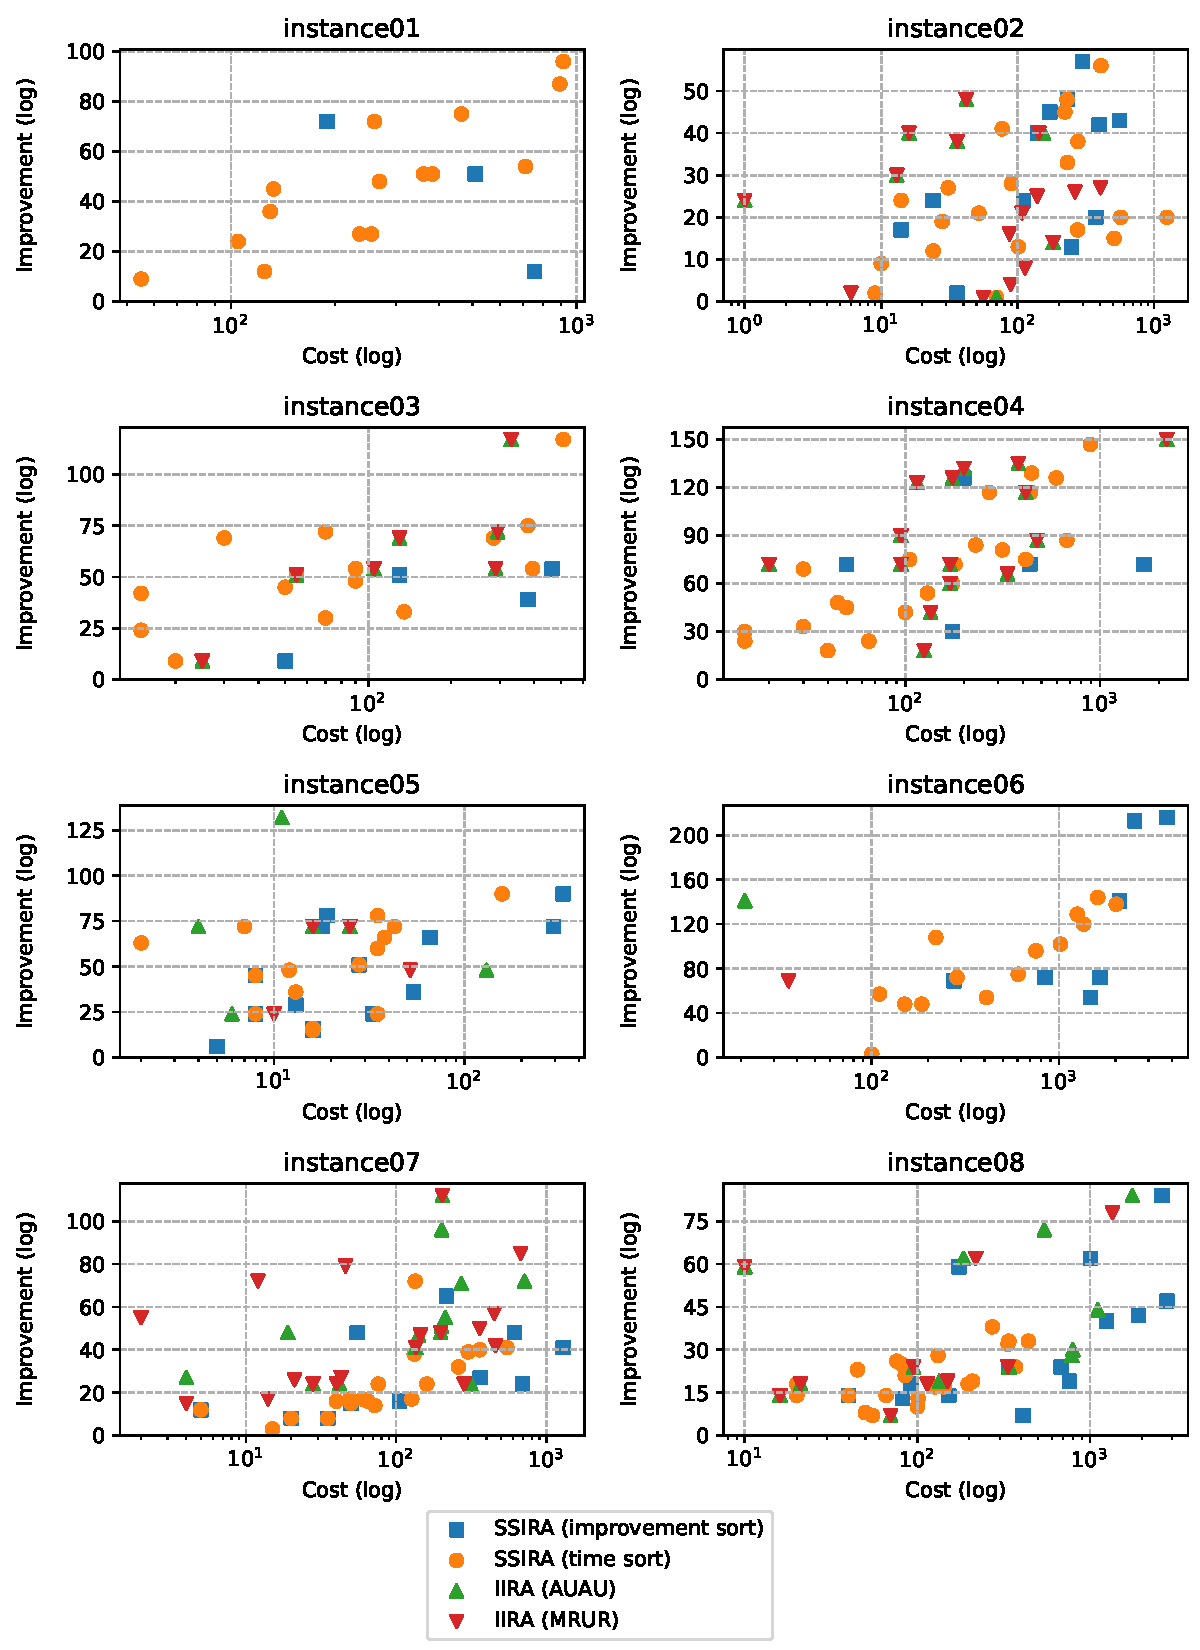
\includegraphics[width=\textwidth]{img/exp_aggregated_cost_improv.pdf}
    \caption{
        Plots for capacity changes costs (x-axis) to achieved improvement (y-axis).
        }
    \label{fig:exp/cost-improv}
\end{figure}

\begin{figure}[t]
    \centering
    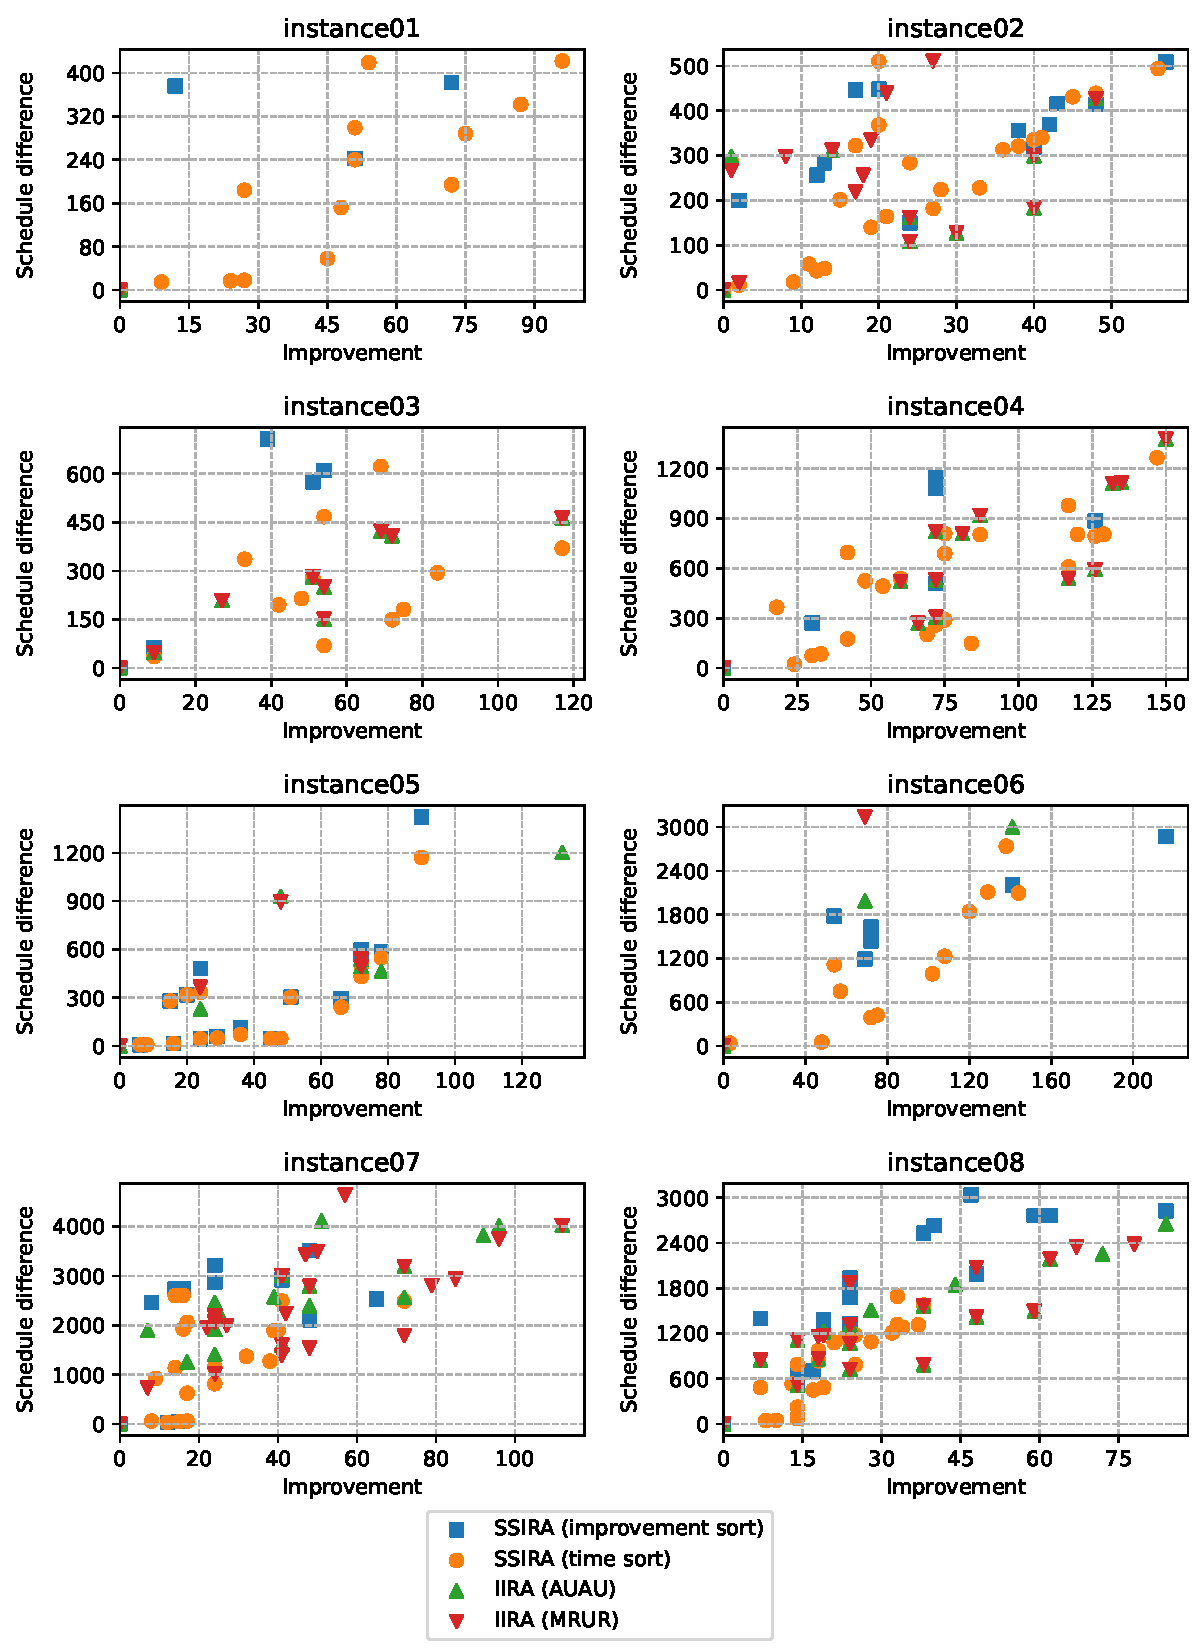
\includegraphics[width=\textwidth]{img/exp_aggregated_improv_diff.pdf}
    \caption{
        Plots for achieved improvement (x-axis) to induced schedule difference (y-axis).
        }
    \label{fig:exp/improv-diff}
\end{figure}

\begin{figure}[t]
    \centering
    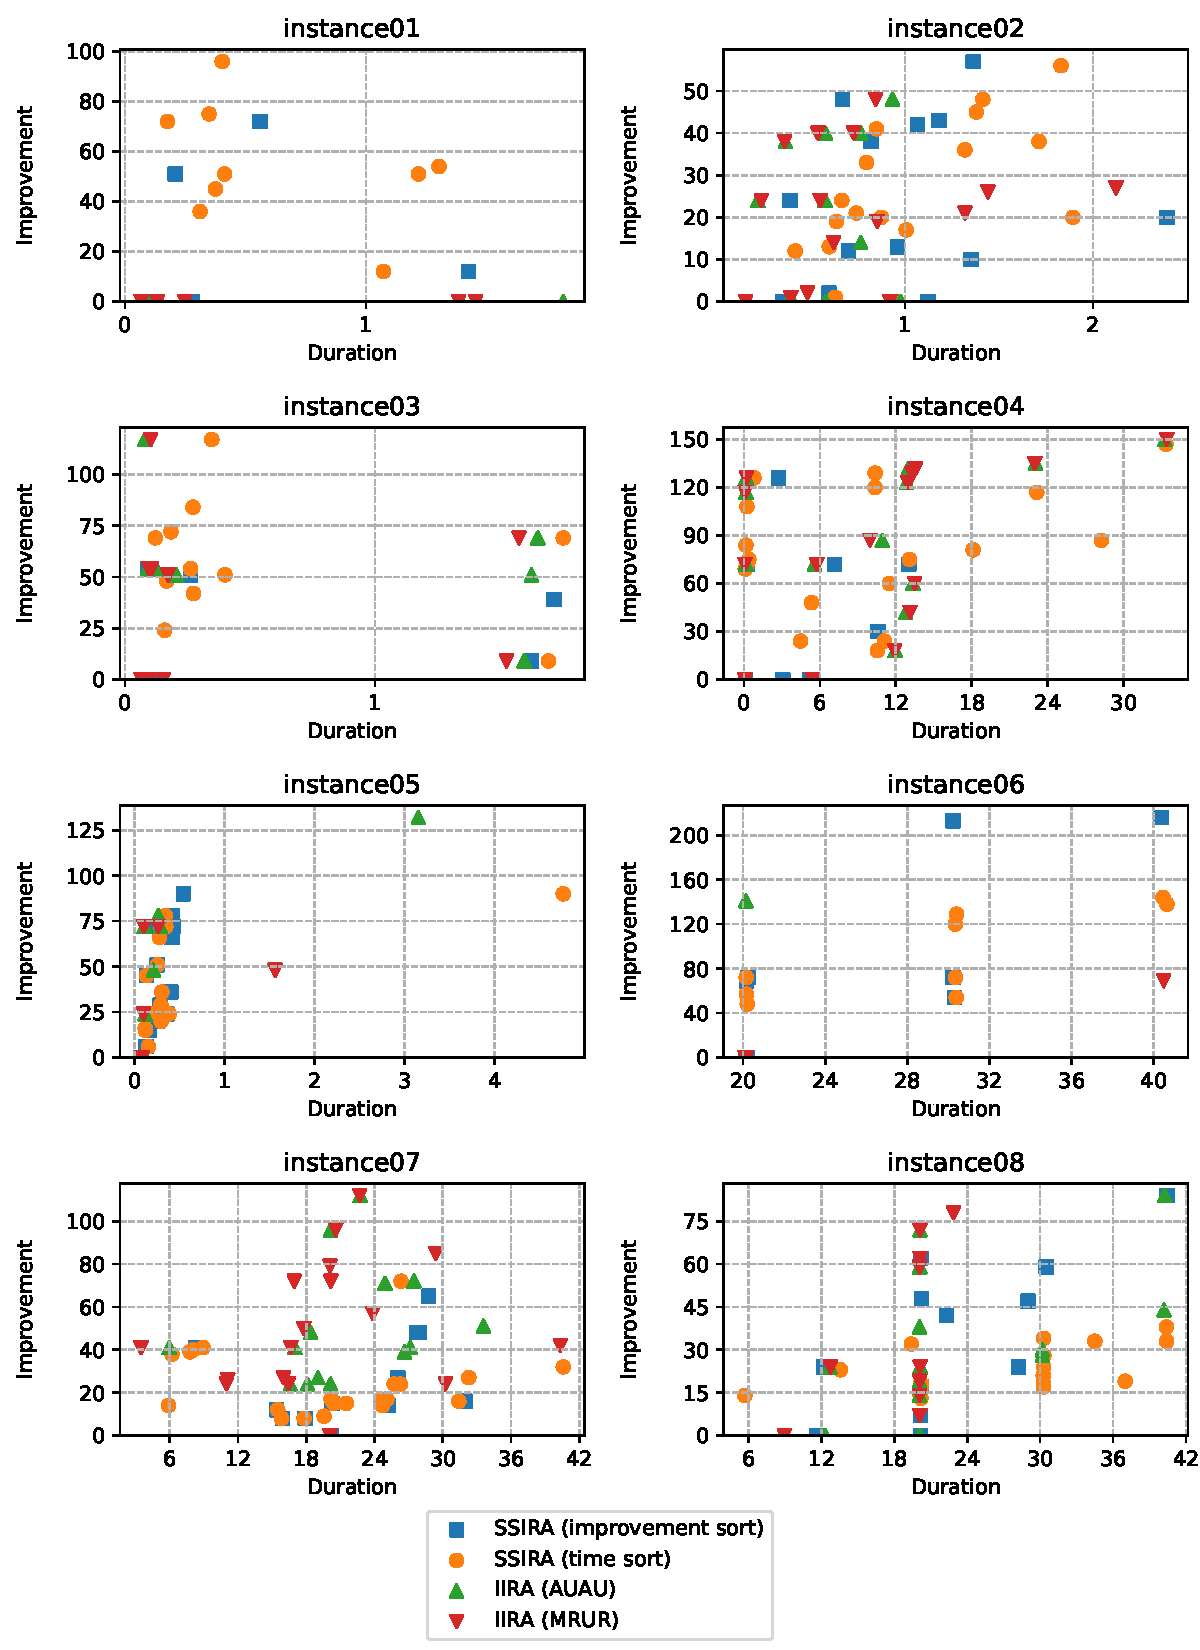
\includegraphics[width=\textwidth]{img/exp_aggregated_duration_improv.pdf}
    \caption{
        Plots for computation time (x-axis) to achieved improvement (y-axis).
        }
    \label{fig:exp/duration-improv}
\end{figure}

\begin{table}[t]
    \centering
    \pgfplotstabletypeset[
        header=true, % Data file contains header
        columns={Instance,{IIRA avg cost per improvement},{IIRA avg improvement per duration},{SSIRA avg cost per improvement},{SSIRA avg improvement per duration}},
        col sep=tab, % Set the column separator to tab
        every head row/.style={
            before row={
            \toprule
            & \multicolumn{4}{c}{\acs{iira}} & \multicolumn{4}{c}{\acs{ssira}} \\
            },
            after row=\midrule,
        },
        every nth row={5[-1]}{
            after row=\midrule,
            },
        columns/Instance/.style={
            string type,
            string replace*={_}{\_},
            column type=l,
            },
        columns/IIRA avg cost per improvement/.style={
            column name=$\mean{\kpiCost / \kpiImprovement}$,
            column type=c,
            fixed, precision=2,
            dec sep align,
            clear infinite,
            },
        columns/IIRA avg improvement per duration/.style={
            column name=$\mean{\kpiImprovement / \kpiDuration}$,
            column type=c,
            fixed, precision=2,
            dec sep align,
            clear infinite,
            },
        columns/SSIRA avg cost per improvement/.style={
            column name=$\mean{\kpiCost/ \kpiImprovement} $,
            column type=c,
            fixed, precision=2,
            dec sep align,
            clear infinite,
            },
        columns/SSIRA avg improvement per duration/.style={
            column name=$\mean{\kpiImprovement / \kpiDuration}$,
            column type=c,
            fixed, precision=2,
            dec sep align,
            clear infinite,
            },
    ]{tabledata/data_kpis.tsv}
    \caption{
        Results concerning the achieved improvement.
        For each algorithm, the~first column represents the average cost per unit of tardiness improvement,
        the~second column represents the average improvement achieved per unit of computation time.
        }
    \label{tab:exp/kpis-improvements}
\end{table}

\begin{table}[t]
    \centering
    \pgfplotstabletypeset[
        header=true, % Data file contains header
        columns={Instance,{IIRA avg diff},{IIRA avg diff per job},{SSIRA avg diff},{SSIRA avg diff per job}},
        col sep=tab, % Set the column separator to tab
        every head row/.style={
            before row={
            \toprule
            & \multicolumn{4}{c}{\acs{iira}} & \multicolumn{4}{c}{\acs{ssira}} \\
            },
            after row=\midrule,
        },
        every nth row={5[-1]}{
            after row=\midrule,
            },
        columns/Instance/.style={
            string type,
            string replace*={_}{\_},
            column type=l,
            },
        columns/IIRA avg diff/.style={
            column name=$\mean{\kpiDiff}$,
            column type=c,
            fixed, precision=2,
            dec sep align,
            clear infinite,
            },
        columns/IIRA avg diff per job/.style={
            column name=$\mean{\kpiDiff} / n$,
            column type=c,
            fixed, precision=2,
            dec sep align,
            clear infinite,
            },
        columns/SSIRA avg diff/.style={
            column name=$\mean{\kpiDiff}$,
            column type=c,
            fixed, precision=2,
            dec sep align,
            clear infinite,
            },
        columns/SSIRA avg diff per job/.style={
            column name=$\mean{\kpiDiff} / n$,
            column type=c,
            fixed, precision=2,
            dec sep align,
            clear infinite,
            },
    ]{tabledata/data_kpis.tsv}
    \caption{
        Results concerning the induced schedule difference.
        For each algorithm, the~first column represents the average schedule difference found for the instance,
        the~second column represents the average difference in start times per job in the instance.
        }
    \label{tab:exp/kpis-difference}
\end{table}

% ~~~~~~~~~~~~~~~~~~~~~~~~~~~~~~~~~~~~~~~~~~~~~~~~~~~~~~~~~~~~~~~~~~~~~~~~~~~~~~~~~~~~~~~~~~~~~~~~~~~~~~~~~~~
\section{Discussion} \label{sec:numerical-experiments/discussion}

\begin{itemize}
    \item \ac{iira} does not consider the target job, it is, however, able to find cheap improvements,
        often better than the \ac{ssira}. \ac{ssira} has a higher chance at finding an improvement.

    \item 
    In \cref{fig:exp/duration-improv}, instances for which the solver time limit might be limiting
    can be identified by apparent groups of solutions all achieving different improvements
    in the same amount of time.
    We could conclude that, on such instances,
    increasing the solver time limit could lead to even better improvements.
    Introducing a solver time limit provides a trade-off between solution quality and computation time,
    especially for more difficult instances.
    However, given that evaluations on most instances were not affected by this time limit,
    we conclude that the time limit was set appropriately in accordance with the difficulty of our problem.
\end{itemize}
